\section{Remastered Audio Identification}

Remastered song identification falls under the domain of cover song identification,
which is a very active area of study in the \ac{mir} community \cite{SerraBook}.
Literature on cover song identification contains different approaches taken to
measure and model music similarity in both symbolic and audio domains. Literature
relevant to cover song identification can be divided into few areas such as
query-by-humming systems, content-based music retrieval, genre classification
and audio fingerprinting.

\vspace{12pt}

In symbolic domain of cover song identification, symbolic representations of
musical content is used in content processing. Query-by-humming systems
\cite{query_by_humming} falls under the symbolic domain as in query-by-humming
systems music contents are stored and processed in symbolic representations.
This query-by-humming method is parallel to retrieving cover songs from a song
database. Even though techniques used in query-by-humming systems could be useful
in future approaches of cover song identification, these systems can't achieve
high accuracy on real world audio music signals \cite{comparative_query_by_humming,SerraBook}.

\vspace{12pt}

Audio domain cover song identification approaches focus on measuring similarity
of music by exploiting music facets shared between two songs. Extracting invariant
features is used to exploit shared music facets. Although such extracted descriptors
are responsible to overcome majority of facet changes, special stress is given for
achieving tempo, key and structure since those facets are not usually managed by
the extracted descriptors themselves \cite{SerraBook}. Hence we can look at existing
literature in terms of feature extraction, tempo invariance, key invariance, structure
invariance and finally similarity comparison. Furthermore, we can take approaches which falls
into this general pipeline (refer Figure \ref{fig:general_pipeline}) to look at different techniques used for these stages and
distinguish each approach from one another by those techniques.

\vspace{12pt}
\begin{figure}[H]
    \centering
    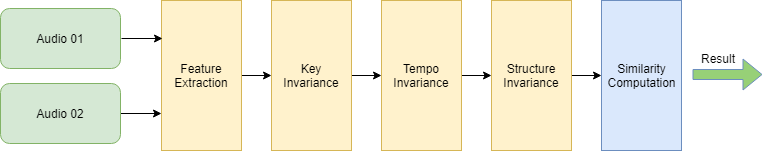
\includegraphics[scale=0.5]{general_pipeline.png}
    \caption{General Pipeline for Cover Song Identification}
    \label{fig:general_pipeline}
\end{figure}
\vspace{12pt}

Bello's cover song identification method extracts chord sequences as the feature and
uses K transpositions for the key invariance. Even though there is no technique used
for structure invariance, \ac{dp} is used for tempo invariance. Finally
it uses edit distance to compute the similarity \cite{Chord}. Since there is no technique
used for structure invariance, that method is inefficient against the structural changes
in cover songs. Egorov proposed another method which uses the same general pipeline with
extracting \ac{pcp} as the feature. But in this method Egorov uses \ac{oti} for key
invariance and \ac{dp} is used for both tempo and structural invariance. And match length
is used for similarity computation \cite{PCP}.

\vspace{12pt}

Foote \cite{Energy} and Izmirli \cite{KeyTemplates} introduced two methods which were using
\ac{dtw} for similarity computation and \ac{dp} for tempo invariance. Both of methods lack
techniques for key invariance and structure invariance which makes those methods to perform
inefficient in both key and temporal changes. The feature extracted by Foote is energy spectrum
while Izmirli extracted key templates. Marlot uses same techniques for tempo invariance and
similarity computation which are \ac{dp} and \ac{dtw}, but melody is the the extracted feature
which using the key estimation for key invariance.

\vspace{12pt}

\begin{table}[H]
    \footnotesize
    \centering
    \begin{tabular}{|l|c|c|c|c|c|}
        \hline
        \multicolumn{1}{|c|}{\textbf{Research}} & \textbf{Feature}                   & \textbf{\begin{tabular}[c]{@{}c@{}}Key \\ Invariance\end{tabular}}  & \textbf{\begin{tabular}[c]{@{}c@{}}Tempo\\ Invariance\end{tabular}} & \textbf{\begin{tabular}[c]{@{}c@{}}Structure\\ Invariance\end{tabular}} & \textbf{\begin{tabular}[c]{@{}c@{}}Similarity\\ Computation\end{tabular}} \\[2ex] \hline
        \textbf{Bello \cite{Chord}}             & \textbf{Chords}                     & \textbf{\begin{tabular}[c]{@{}c@{}}K\\ transpositions\end{tabular}}  & \textbf{DP}                        & \textbf{}                          & \textbf{\begin{tabular}[c]{@{}c@{}}Edit\\ distance\end{tabular}} \\[2ex] \hline
        \textbf{\begin{tabular}[c]{@{}l@{}}Egorov \& \\ Linetsky \cite{PCP}\end{tabular}}      & \textbf{PCP}                        & \textbf{OTI}                        & \textbf{DP}                        & \textbf{DP}                        & \textbf{\begin{tabular}[c]{@{}c@{}}Match\\ length\end{tabular}} \\[2ex] \hline
        \textbf{Foote \cite{Energy}}            & \textbf{\begin{tabular}[c]{@{}c@{}}Energy \\ spectral\end{tabular}} & \textbf{}                           & \textbf{DP}                        & \textbf{}                          & \textbf{DTW}                       \\[2ex] \hline
        \textbf{Izmiril \cite{KeyTemplates}}    & \textbf{\begin{tabular}[c]{@{}c@{}}Key \\ templates\end{tabular}} & \textbf{}                           & \textbf{DP}                        & \textbf{}                          & \textbf{DTW}                       \\[2ex] \hline
        \textbf{Marolt \cite{Melody}}           & \textbf{Melody}                     & \textbf{\begin{tabular}[c]{@{}c@{}}Key \\ estimation\end{tabular}} & \textbf{DP}                        & \textbf{}                          & \textbf{DTW}                       \\[2ex] \hline
    \end{tabular}
    \caption{Cover song identification methods and their techniques used for each step in general pipeline}
    \label{tab:literature}
\end{table}

\vspace{12pt}

Related works mentioned above for audio domain can be modelled to the general pipeline for cover
song identification (refer Figure \ref{fig:general_pipeline}) as described in Table \ref{tab:literature}.